\section{Experiments}

In this section, we conducted corresponding experiments in the D4RL public datasets and the real-world recommendation system scenarios. Our primary points of comparison are reward modification strategies include: scale, return min-max, average, ensemble. Furthermore, these strategies can be combined with any offline RL algorithms without extra efforts, model-free offline RL algorithms BC, CQL and model-based algorithm MOPO are included depend on the environment as follows:

\begin{itemize}
    \item Behaviour Cloning(BC). BC uses supervised learning for policy learning, and the learning process does not depend on the rewards. Therefore, delaying the rewards has no effect on its policy learning process. In this part, we directly quote the results published in the D4RL paper.
    
    \item Conservative Q-Learning(CQL). CQL is a type of model-free algorithm. It learns a Q-value function directly from the data, thereby avoiding action out of distribution(OOD) caused by offline reinforcement learning.
    
    \item Model-based Offline Policy Optimization(MOPO). MOPO is a model-based algorithm. It first learns multiple supervised learning models (including state transition and reward function) from offline data, and the strategy interacts with the learned model. The reward adds an additional transition to the joint model. Deterministic estimation, as an empirical reward Lower Bound, has verified its effectiveness in theory and experiment.
    
\end{itemize}

we verify the effectiveness of aforementioned methods in solving the delayed rewards problems. Experiments conducted both on simuated offline datasets (OpenAI Gym) and customized real-world datasets. All tasks involves delayed rewards and high-dimensional observation spaces, xxx.

\subsection{Evaluation on D4RL public datasets}

In this section, we compare to BC, CQL, and MOPO on three continuous control tasks from the D4RL bechmark. As the original datasets We first construct the delay rewards datasets from the original none-delayed rewards datasets on 4 levels setting:

\begin{enumerate}
    \item Random: 1 million timesteps generated by a “random” policy.
    \item Medium: 1 million timesteps generated by a “medium” policy that achieves approximately one-third the score of an expert policy.
    \item Medium-Replay: the replay buffer of an agent trained to the performance of a medium policy (approximately 25k-400k timesteps in our environments).
    \item Medium-Expert: 1 million timesteps generated by the medium policy concatenated with 1 million timesteps generated by an expert policy.
\end{enumerate}

\textbf{Datasets construction.} In order to make a public comparison with other offline algorithms, we delay the dense reward based on the D4RL gym datasets. Specifically, we perform constant delay setting: we set a hyper-parameter $K$ as the delay interval which controls the sparsity of the delayed rewards. We set the delayed reward at equal intervals with $K$ as the un-discounted cumulative rewards of corresponding interval, the missing reward filled with 0, formally:

For a trajectory $\tau$ with length $T$, we set the delayed reward of time step $t$ as $r_t^{delay}$, where:

$$
\begin{aligned}
r_t^{delay} = \begin{cases}
0, \text{if} \ t \mod K \neq 0; \\
\sum_{i = t - K + 1}^t r_t, \text{otherwise}.
\end{cases}
\end{aligned}
$$

Such construction strategy introduce sparsity to delay rewards, meanwhile, it keeps the rule that for any trajectory in the original datasets, the un-discounted cumulative rewards keep constant before and after the operation, mathematically, we have:

$$
\sum_{t = 1}^{T} r_t = \sum_{t = 1}^{T} r_t^{delay}
$$

To facilitate intuitive and clear comparison of the delay reward:
\begin{figure}[H]
    \centering
    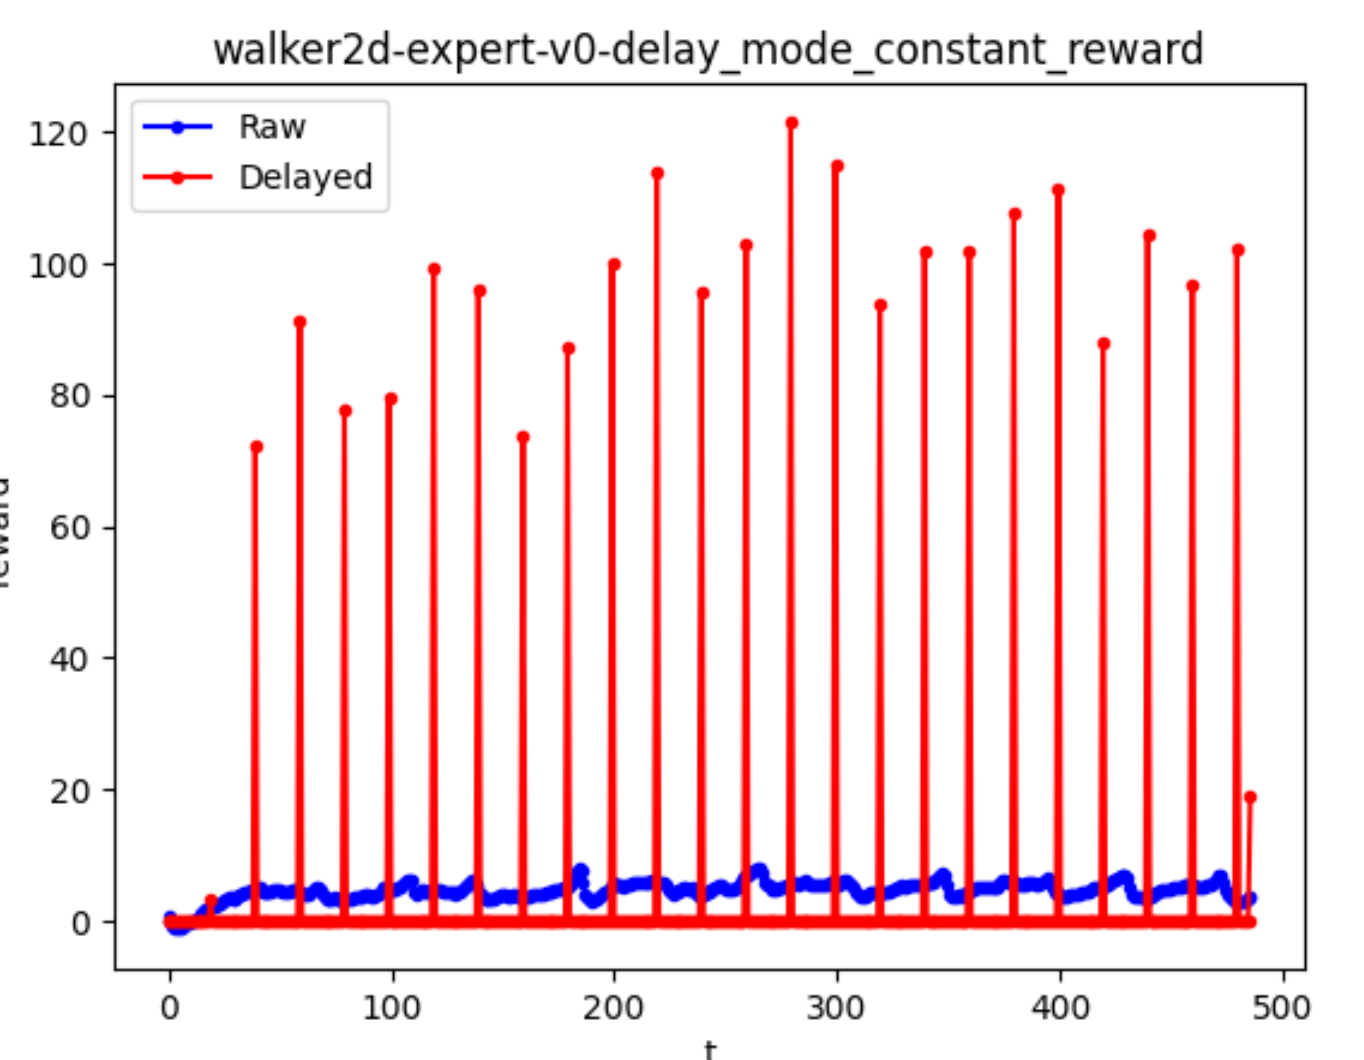
\includegraphics[width=0.95\textwidth]{assets/image.png}
    \caption{Delayed rewards xxx}
    \label{fig:fig1}
\end{figure}


We compare to BC, CQL, and MOPO. BC numbers are reported from the original D4RL paper, CQL and MOPO results are run by us. Our results are shown in Table 1. MOPO(average) achieves the highest scores in 11/12 of the tasks.


\begin{table*}[h]
\centering
\begin{tabular}{lll|cc|ccc}
\toprule
& & & & & \multicolumn{3}{c}{\bf MOPO} \\
\multicolumn{1}{l}{\bf Dataset} & \multicolumn{1}{c}{\bf Environment} & \multicolumn{1}{c|}{\bf Delay} & \multicolumn{1}{c}{\bf BC} & \multicolumn{1}{c|}{\bf CQL} & \multicolumn{1}{c}{\bf{Normal}} & \multicolumn{1}{c}{\bf +Average} & \multicolumn{1}{c}{\bf +Ensemble}\\
\midrule
Random        & HalfCheetah &  20 & $2.1$ &  -  &  $0.1$ &  $\bf{25.3 \pm 1.5 }$ \\
Random        & Hopper      &  20 & $1.6$ &  -  &  $3.1$ &  $\bf{9.1 \pm 1.5 }$ \\
Random        & Walker2d    &  20 & $9.8$ &  -  &  $0.1$ &  $\bf{12.6 \pm 6.1 }$ \\
\midrule
Medium        & HalfCheetah &  20 & $36.1$ &  - &  $-0.8$ &  $\bf{48.3 \pm 2.4}$ \\
Medium        & Hopper      &  20 & $29$ & - & $5.1$ &  $19.0 \pm 8.1$ \\
Medium        & Walker2d    &  20 & $6.6$ & - & $4.5$ &  $\bf{72.3 \pm 0.9}$ \\
\midrule
Medium-Replay & HalfCheetah &  20 & $38.4$ & - & $1.9$ &  $54.5 \pm 3.2$ \\
Medium-Replay & Hopper      &  20 & $11.8$ & - & $1.9$ &  $89.8 \pm 5.7$ \\
Medium-Replay & Walker2d    &  20 & $11.3$ & - & $0.9$ &  $\bf{59.1 \pm 3.7}$ \\
\midrule
Medium-Expert & HalfCheetah &  20 & $35.8$ & - & $2.1$ &  $\bf{73.6 \pm 8.3}$ \\
Medium-Expert & Hopper      &  20 & $111.9$ & - & $9.4$ &  $\bf{22.1 \pm 3.2}$ \\
Medium-Expert & Walker2d    &  20 & $6.4$  & - & $6.8$ & $\bf{99.0 \pm 3.7}$\\
\bottomrule
\end{tabular}
\caption{
Results for D4RL datasets\protect\footnotemark.
We report the mean and variance for three seeds.
MOPO+Average outperforms conventional RL algorithms on almost all tasks.}
\label{tbl:mujoco_results}
\end{table*}

\subsection{Evaluation on recommender system simulated datasets}
In order to verify the effectiveness of the reward modification strategy proposed in the article, we added a simulation environment in a real-world scenario for verification.



